\section{My first underground camp trip - discovery of `\passage{Shithole}'}
After numerous carries and three progressively tougher bounce trips, I was physically and
mentally prepared for my first underground camping trip. After probably forgetting some of my kit and faffing on the surface the time had come to enter the abyss, an abyss now more familiar to me. On both my underground camp trips I was surprised by the relative ease of getting to camp compared to the demanding ascents on the way up. 

\margininbox{Shithole}
{\begin{itemize}
	\item Benjamin Honan
	\item Oliver Myerscough
\end{itemize}}

After reaching camp we were met by Rhys and James who had explored `100's of meters of walking passage'. Initially I thought they were joking, having heard Rhys going on about finding walking passage past a lead in Yorkshire on countless previous occasions. But it was true! Needless to say I was impressed and congratulated the humble team.

During my first UG camping experience, the dark environment seemed familiar but also psychologically counter-intuitive. It seemed strange that if I were to misplace my head-torch after waking up, that I would have no alternate means to "switch on the lights". 

Oli had told me there was a lead close to camp which would be a good first pushing experience. After a short climb and some rapid descents, we reached \passage{Falls Road}. We explored one of the "leads" for a bit but soon realised that there wasn't any realistic opportunity for discovery at the far reaches of \passage{Falls road}. Everything became far too narrow. The second lead was a short squeeze which was preceded by a short traverse. We initially couldn't figure out how the traverse was done in the past. There was one acrobatically placed sling around a natural but other than that, there were no bolts. \bignote{Oli and I were not as suicidal as whoever placed that sling and decided that we needed to place a few hand bolts}. We forgot the bolting kit and Oli decided to quickly go back to camp by himself to fetch it. 

During this brief period of solitude, the psychological strangeness of the experience hit me again. I couldn't help myself to make out the sounds of distant voices in the echoing drips of water that occupied my attention. I kept on thinking that Oli was calling to me and I was almost convinced to respond either by going back or shouting.

The arduous, labour intensive nature of hand bolting was soon revealed to me. Oli suggested I do my best to keep myself warm to prevent the onset of hypothermia whilst I waited for him to place the bolts. After maybe an hour I was starting to get quite cold. 

After passing the traverse, the lead was clear. A very tight squeeze. The squeeze seemed promising as there was quite an echo beyond it, however we decided to return to the squeeze the next day as at least I wasn’t in the mood for tight spaces. \bignote{When we returned to underground camp we listened to Blackadder non-stop and munched on some delicious fish and cheddar noodles}. The night was cold. 

The next morning we pushed a lead a bit further on in the cave (I forget the location) \sidenote[][-100pt]{This was the Hotpants crawl, later pushed by Jim Evans and Dave Kp} and spent quite a lot of time hammering at the walls of a very tight tube. I kept imagining the prospect of rocks falling on me whilst in the tight tube at 600m underground. I wasn’t that keen to continue pushing it, I don’t think there was much of a draught anyway. We left and returned to the previous day’s echoey squeeze. 

After taking my SRT kit off, I managed to wriggle my way through the obstruction, and… wow! It was really quite an impressive chamber, about twice the cross sectional area of caving stores and about as high as the Union building. But alas, there was no draught or anywhere to continue, so this was it. 


\begin{marginfigure}
	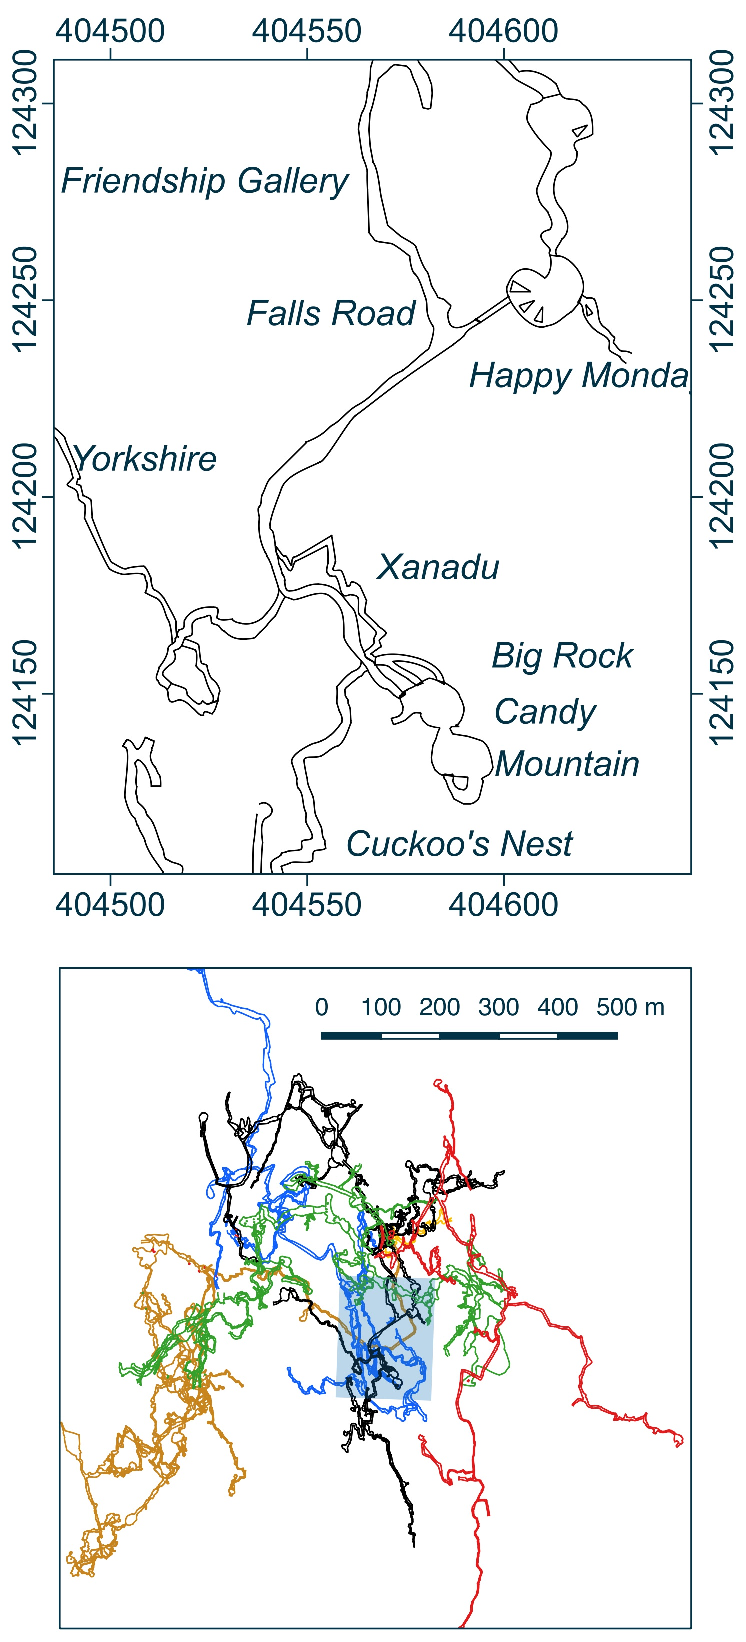
\includegraphics[width= \linewidth]{images/little_insets/bigrock_high_inset.pdf}
	\caption*{Plan view of \protect\passage{Falls Road}--- Slovenian National Grid EPSG 3794}
	\label{Falls Road}
\end{marginfigure}

There was something interesting about this place though - on a spikey stalagmite about 3m above the ground were the remnants of a plastic biodegradable bag - a shit bag which ended up being the namesake of our find, \passage{Shithole}. Back at camp we listened to more Blackadder and had more cheesy, fishy noodles, hmmm…

The next morning was an early start to make sure we didn’t miss our call out. I remember it taking about 6 hours to get to the surface, we sang the Blackadder theme tune the whole way out: `Black Aaaadder, Black Aaaaadder, na na na na na naaaaaaa, ...'.

\name{Ben Honan}

